\documentclass{article}
\usepackage{graphicx, amsmath, amssymb, enumerate, microtype, titlesec, xfrac, xcolor, mathtools, multicol, mathrsfs}
\usepackage[italicdiff]{physics}
\usepackage[bookmarks=false]{hyperref}
\hypersetup{
    colorlinks=true,
    linkcolor=[RGB]{59 108 209},
    urlcolor=[RGB]{59 108 209}
}
\urlstyle{same}
\DisableLigatures{encoding= *, family=*}
\setcounter{secnumdepth}{4}
\newcommand{\nsum}[1][1.4]{% only for \displaystyle
    \mathop{%
        \raisebox
            {-#1\depthofsumsign+1\depthofsumsign}
            {\scalebox
                {#1}
                {$\displaystyle\sum$}%
            }
    }
}
\newlength{\depthofsumsign}
\setlength{\depthofsumsign}{\depthof{$\sum$}}
\newlength{\totalheightofsumsign}
\newlength{\heightanddepthofargument}
\def\tmp#1 #2\relax{#1}
\setbox0=\hbox{$\xdef\intfont{%
    \expandafter\tmp\fontname\textfont3\expandafter\space\space\relax}$}
\font\tmp=\intfont\space at10pt\relax
\setbox0=\hbox{$\textfont3=\tmp \displaystyle \int$}
\dimen0=\ht0 \advance\dimen0 by\dp0 \divide\dimen0 by10 
\xdef\intsize{\the\dimen0}
\def\dividedimen (#1/#2){\expandafter\ignorept\the
   \dimexpr\numexpr\number\dimexpr#1\relax
   *65536/\number\dimexpr#2\relax\relax sp\relax
}
{\lccode`\?=`\p \lccode`\!=`\t  \lowercase{\gdef\ignorept#1?!{#1}}}
\def\flexibleint{\def\fxintL{}\def\fxintU{}\futurelet\next\fxintA}
\def\fxintA{\ifx\next_\expandafter\fxintB\else\expandafter\fxintC\fi}
\def\fxintB_#1{\def\fxintL{#1}\fxintC}
\def\fxintC{\futurelet\next\fxintD}
\def\fxintD{\ifx\next^\expandafter\fxintE\else\expandafter\fxintF\fi}
\def\fxintE^#1{\def\fxintU{#1}\fxintF}
\def\fxintF#1{\begingroup
   \setbox0=\hbox{$\displaystyle{#1}$}%
   \dimen0=\ht0 \advance\dimen0 by\dp0
   \setbox1=\hbox{$\vcenter{\copy0}$}%
   \font\tmp=\intfont\space at\dividedimen(\dimen0/\intsize)pt
   \lower\dimexpr\dp0-\dp1\hbox{%
      $\textfont3=\tmp \displaystyle\int_{\fxintL}^{\fxintU}$}
   \box0
   \endgroup
}
\newcommand*\fullcirc[1][0.3ex]{\tikz\fill (0,0) circle (#1);} 
\titleformat{\paragraph}
{\normalfont\normalsize\bfseries}{\theparagraph}{1em}{}
\titlespacing*{\paragraph}
{0pt}{3.25ex plus 1ex minus .2ex}{1.5ex plus .2ex}
\title{Definite Integration Doubts}
\author{}
\date{}

\begin{document}
\maketitle

\section*{}
\begin{enumerate}[$\mathcal{D}$1.]
   \item $$\displaystyle\int_{-1}^{1} \dv{x}(\tan^{-1} \dfrac{1}{x} ) \, dx $$
Why isn't the above integral equal to $\displaystyle\int_{-1}^{1} d\left(\tan^{-1} \dfrac{1}{x} \right)=\biggl[\tan^{-1} \dfrac{1}{x}\biggr]_{-1}^{1}=\dfrac{\pi}{2} $
   \item Consider, $$I=\displaystyle\int_{-1}^{1} \sqrt{1+x^2} \, dx $$
   Let, $u=1+x^2 \implies du \, =2x \, dx$ \\
   also, $x=-1 \implies u = 2, x=1 \implies u = 2$\\
   Now, $I$ becomes, $$\displaystyle\int_{2}^{2} \dfrac{\sqrt{u}}{2 \sqrt{u-1}} \, du $$
   Since, upper limit and lower limit are same, $$\boxed{I=0}$$
   But from graph, 
   $$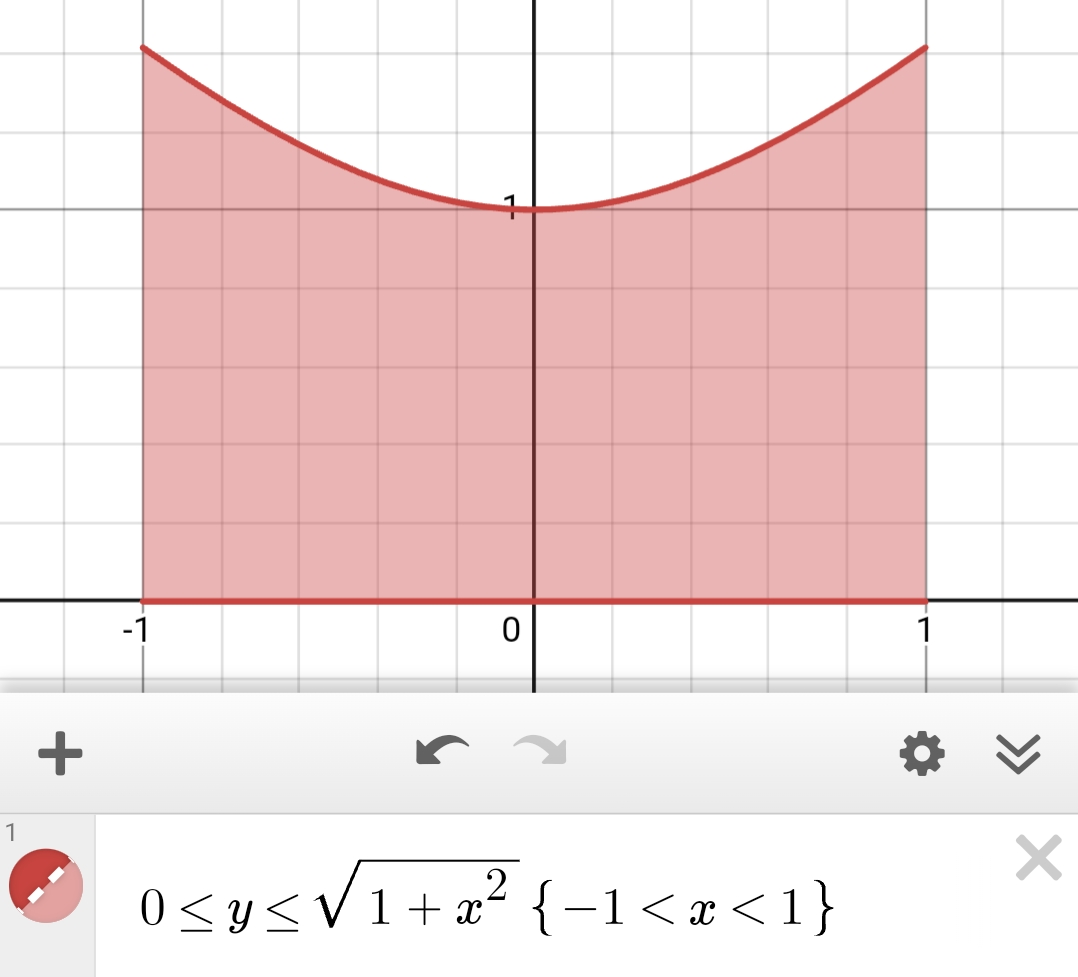
\includegraphics[scale=0.1]{D2.jpg}$$
   Red region represents $I$, Clearly, $I>0$\\
   Why is this substitution wrong?
   \item How to evaluate $\displaystyle\int_{0}^{a} \lfloor x^n \rfloor \, dx  \hspace{2mm}$ ? 
\end{enumerate}
\end{document}